\begin{frame}{Kiến trúc tích hợp đàm thoại thời gian thực (Voice Agent)}
\begin{figure}[H]
\centering
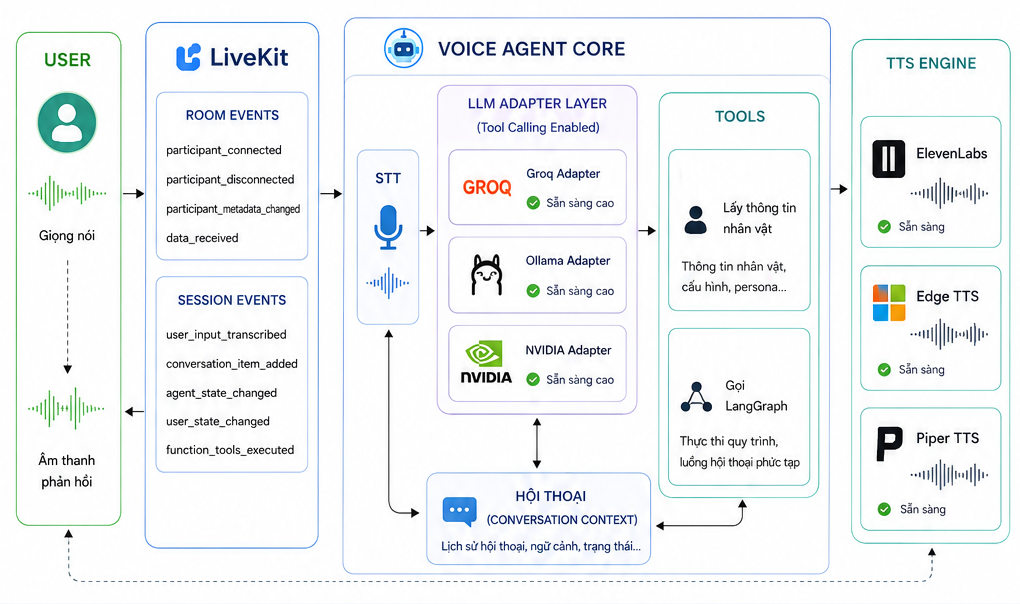
\includegraphics[height=0.7\textheight,width=0.9\textwidth,keepaspectratio]{pictures/voice-livekit-overview.png}
\caption{Sơ đồ tích hợp LiveKit đàm thoại giọng nói}
\end{figure}

\note{
Hệ thống tích hợp máy chủ LiveKit để cung cấp tính năng đàm thoại giọng nói thời gian thực với trợ lý ảo.
Khi người dùng kết nối, Voice Agent hoạt động như một LiveKit Agent, chủ động kết nối và trao đổi âm thanh hai chiều thông qua giao thức WebRTC. Voice Agent tích hợp các mô hình VAD (phát hiện giọng nói), STT (chuyển giọng nói thành văn bản), LLM (suy luận phản hồi) và TTS (chuyển văn bản thành giọng nói) với độ trễ cực thấp.
}
\end{frame}
